\documentclass{article}
\usepackage[utf8]{inputenc}
\usepackage{fullpage}
\usepackage{amsmath, mathtools}
\usepackage{amsfonts}
\usepackage{amssymb}
\usepackage{graphicx}
\usepackage{colortbl}
\usepackage{xr}
\usepackage{hyperref}
\usepackage{longtable}
\usepackage{xfrac}
\usepackage{tabularx}
\usepackage{float}
\usepackage{siunitx}
\usepackage{booktabs}
\usepackage{caption}
\usepackage{pdflscape}
\usepackage{afterpage}
\usepackage{seqsplit}
\usepackage{underscore}
\usepackage{lscape}
\usepackage[english]{babel}
\usepackage[T1]{fontenc}


% For easy change of table widths
\newcommand{\colZwidth}{1.0\textwidth}
\newcommand{\colAwidth}{0.13\textwidth}
\newcommand{\colBwidth}{0.82\textwidth}
\newcommand{\colCwidth}{0.1\textwidth}
\newcommand{\colDwidth}{0.05\textwidth}
\newcommand{\colEwidth}{0.8\textwidth}
\newcommand{\colFwidth}{0.17\textwidth}
\newcommand{\colGwidth}{0.5\textwidth}
\newcommand{\colHwidth}{0.28\textwidth}


\newcommand{\deftheory}[9][Not Applicable]
{
\newpage
\noindent \rule{\textwidth}{0.5mm}

\paragraph{RefName: } \textbf{#2} \phantomsection 
\label{#2}

\paragraph{Label:} #3

\noindent \rule{\textwidth}{0.5mm}

\paragraph{Equation:}

#4

\paragraph{Description:}

#5

\paragraph{Notes:}

#6

\paragraph{Source:}

#7

\paragraph{Ref.\ By:}

#8

\paragraph{Preconditions for \hyperref[#2]{#2}:}
\label{#2_precond}

#9

\paragraph{Derivation for \hyperref[#2]{#2}:}
\label{#2_deriv}

#1

\noindent \rule{\textwidth}{0.5mm}

}

\begin{document}

\title{
Software Requirements Specification for ParkingLotHawk \\
  \large MECHTRON 4TB6 Capstone Design Project 
    }

\author{\authname Team \#34 \\
Fady Zekry Hanna, zekryhf \\
Winnie Trandinh, trandint \\
Muhammad Ali, alim102 \\
Muhammad Khan, khanm120}

\date{\today}
	
\maketitle

~\newpage

\pagenumbering{roman}

\tableofcontents

~\newpage

\section*{Revision History}

\begin{tabularx}{\textwidth}{p{3cm}p{2cm}X} 
\toprule {\bf Date} & {\bf Version} & {\bf Notes}\\
\midrule
Oct 5, 2022 & 1.0 & Team Finalized SRS\\

\bottomrule
Oct 31, 2022 & 2.0 & Split up Autonomous Move and malfunction states, added transition requirement and performance requirements accordingly with bidirectional references - did not update state machine pictures, state transition table and traceability tables. Also added USE\_005 which may require new references. Added new input, m\_CompulsiveMove. Added hover state lock. Removed 90\% exploration requirement. 
\\

\bottomrule
\end{tabularx}

~\newpage

\pagenumbering{arabic}

\section{Introduction}
\label{sec:Intro}
\subsection{Purpose}
The purpose of the project will be to design an aerial drone, called ParkingLotHawk, that can detect how many parking spots are available in any given parking lot. ParkingLotHawk can be operated by property personnel to communicate to drivers on how many spots are available at a parking lot. ParkingLotHawk will explore over any parking lot designated by the user and will aggregate visual information and output the amount of parking spots available. Many parking lots today do not have this data and this data can be used for many reasons. The data can be used by retailers to know how long customers stay at specific stores or location. This data can also be used for drivers to know if there are parking spots available in a specific location allowing for drivers to not waste time and resources in a full parking lot. 
\subsection{Scope}
The product specified in this SRS \ref{DefTable} is about an autonomous aerial drone for helping parking lot operators understand the state of their parking lot. The product specified does not require the operator to manually control or move the drone, rather the requirement describes various autonomous flight modes. The specified drone shall support the ability to both create a path to reach its specified location, as well as create and follow a path to explore large parking lot sections autonomously. During flight, the specified drone shall transmit live information about the parking lot sections it detects. The completed product, a combination of the physical drone and any equipment/application intended to be kept by the parking lot operator to communicate with the drone, is called the ParkingLotHawk. A solution that implements the requirements will help parking lot authorities of outdoor lots quickly gain valuable information without requiring permanent solution, large monetary and time investments, or complex training. 



\subsection{Definitions, Acronyms, and Abbreviations}

\begin{table}[!h]
\begin{center}
\caption {Key terms, acronyms, and abbreviations are defined.} 
\label{DefTable}
\begin{tabular}{ | m{3cm} | m{11cm} | }
\hline
Term & Definition. \\
\hline
Inclement Weather & Weather with rain, snow, fog, and/or winds over 50 km/hour. \\
\hline
Parking Lot Authorities & Event organizers for whome parking lot management is one of thier tasks. Examples include property managers, and concert organizers.  \\
\hline
Parking Lot Operator (Operator) & Person responsible for managing the product during operation. \\
\hline
Clear Boundaries & The border surrounding the parking lot. For example the border between the lot and sidewalks, buildings, curbs, and sections of grass.\\
\hline
Flight Controller & The central part of the drone that receives most sensor input and is responsible for controlling the propellers.\\
\hline
Flight States & The states of the state machine that require the drone to be aerially flying, detailed in the requirements \ref{flightModes}.\\
\hline
PC & Personal Computer. \\
\hline
MVP & Minimum Viable Product. \\
\hline
SRS & Software Requirement Specifications. \\
\hline
DMS & Degrees/Minutes/Seconds used as GPS coordinates\\
\hline
\end{tabular}
\end{center}
\end{table}

\subsection{References}
There are no external software documents referenced in the SRS. 

\subsection{Overview}
The SRS is organized to follow the IEEE 1998 template. \nameref{sec:Intro} contains the purpose of the SRS as well as the scope of the product and the problem it solves. \nameref{sec:Desc}  refines the scope of the product further. It provides more detail about the products environment, primary functions, intended users, constraints, and finally assumptions. \nameref{sec:Req} contains a detailed description of all requirements, organized into sections for readability. Finally, the \nameref{appendix} contains \nameref{appendixa} regarding new knowledge and skills the team needs to create the specified product, along with approaches to how the team will acquire the knowledge. The \nameref{appendixb}  also contains the formal transition tables between the states of the finite state machine which will be later introduced within \nameref{subsec:ProdFunc}.
\section{Overall Description}
\label{sec:Desc}
General factors that affect the product and the requirements are described in the following subsections. A high-level overview of the product functions are also described (see \nameref{subsec:ProdFunc}). 
\subsection{Product Perspective}
The system specified is an independent and stand-alone parking lot tool. It does not fit into or interface with a larger system of parking lot and security technologies the operator may have available. 

The environment consists of an outdoor parking lot and the operator's PC. The operator's PC shall be operating with Windows 10 or Windows 11.

\subsection{Product Functions}
\label{subsec:ProdFunc}
This subsection describes the behaviour overview of the ParkingLotHawk by splitting its functionality into various interconnected states of operation. These states are shown within the \nameref{InfFSM} and are further refined within \nameref{sec:funcReqs}. 
\subsubsection{Idle State}
\label{Idle State}
The product is powered on and communicating with the operator application, but all motors are turned off. 
\subsubsection{Hover State}
\label{Hover State}
The product maintains its current longitudinal and latitudinal position, and hovers at a pre-defined operator selected height. 
\subsubsection{Autonomous Move State}
\label{Autonomous Move State}
If the Operator requests to move to a specific location within the parking lot, the product shall move to that location and hover at a pre-defined operator-selected height. Note that this height does not need to be the same as the height specified in the Hover State. 
\subsubsection{Compulsive Move State}
\label{Compulsive Move State}
If the Operator requests to move to a location, the product shall move to that location regardless of if it is within the parking lot. One at that location the product shall hover at a pre-defined operator-selected height. Note that this height does not need to be the same as the height specified in the Hover State. 
\subsubsection{Autonomous Explore State}
\label{Autonomous Explore State}
The product shall autonomously explore within the current parking lot without operator input. 
\subsubsection{Configure State}
\label{Configure State}
During this state, the operator is able to define parameters of operation that are not configurable in other states. 
\subsubsection{Off State}
\label{Off State}
The product shall be unpowered and stops communication with the operator application. 
\subsubsection{Land State}
\label{Land State}
The product shall land at its initial launch location.
\subsubsection{Desired Location Error State}
\label{Desired Location Error State}
This error state occurs when the operator specifies an invalid desired position and shall provide the appropriate error message to the operator. 
\subsubsection{No Parking Lot Detected Error State}
\label{No Parking Lot Detected Error State}
This error state occurs when the product does not detect a valid parking lot, and shall provide the appropriate error message to the operator.
\subsubsection{Malfunction State}
\label{Malfunction State}
This error state occurs when an internal/external malfunction occurs in such a way that nominal performance is not possible. The resulting action by the product will be further specified within \nameref{sec:funcReqs}. 
\subsubsection{Communication Lost State}
\label{Communication Lost State}
This error state occurs when the product has lost connection or has a very weak connection so the Operator's Application, and shall provide the appropriate error message to the operator.
\subsubsection{Arm State}
\label{Arm State}
During this state the drone shall arm and remain armed.
\subsubsection{Takeoff State}
\label{Takeoff State}
During this state, the vehicle shall take off the ground towards m\_MaxHoverHeight.

The normal modes of operation include the following:
\begin{itemize}
  \item Idle State
  \item Hover State
  \item Autonomous Move State
  \item Compulsive Move State
  \item Autonomous Explore State
  \item Configure State
  \item Off State
  \item Arm State
  \item Takeoff State
\end{itemize}
The flight modes of operation \label{flightModes} include the following:
\begin{itemize}
  \item Hover State
  \item Takeoff State
  \item Autonomous Move State
  \item Compulsive Autonomous Move
  \item Autonomous Explore State
   \item No Parking Lot Detected Error State
   \item Desired Location Out of Bounds Error State
\end{itemize}
With the exception of the Configure State and Off State, the product shall update continuously update c\_CurrentView and c\_OccupancyMap for the operator. These requirements are further refined within \nameref{sec:funcReqs}. 

The error modes are listed below:
\begin{itemize}
    \item Desired Location Error State
    \item No Parking Lot Detected Error State
    \item Malfunction State
    \item Communication Lost State
\end{itemize}
These modes are used to handle errors either from the operator, or internally from the product. 

The behaviour overview of the product is described below, with each directional arrow representing a transition between states:
\begin{figure}[h!]
  \begin{center} 
  \caption{Informal Finite State Machine Diagram } 
  \label{InfFSM}
 
        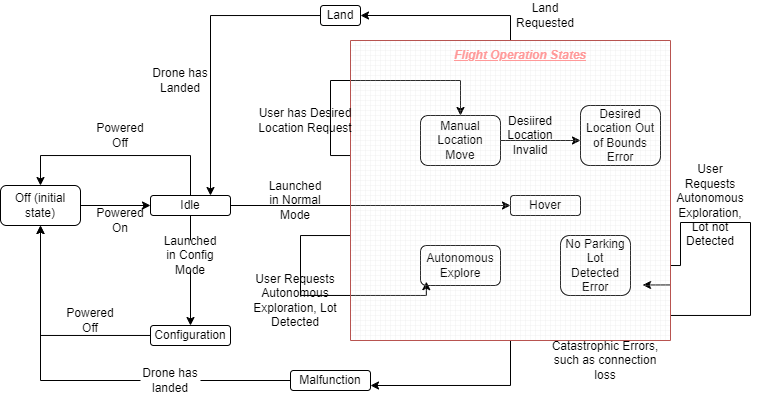
\includegraphics[width=0.5\textwidth]{InformalFSM.png}
  \end{center}
\end{figure}

\subsection{User characteristics}
The stakeholders are Dr. Spencer Smith, the MECHTRON 4TB6 teaching assistants, parking lot authorities \ref{DefTable}, parking lot operators, and visitors of the parking lot. All demographics mentioned would find the data of the ParkingLotHawk useful. There is no technical or software knowledge expected for users of the ParkingLotHawk. The user will need to turn the drone on and place it close to a parking lot.  The ParkingLotHawk is made mindful of the societhttps://www.overleaf.com/project/633da9268221bf16bb108961y and community and its health impacts; therefore, little to no air or noise pollution shall occur, and no invasion of privacy shall ensue.
\subsection{Constraints}
\label{sec:Constraints}
The purpose of the system is to provide parking lot information to parking lot operators, who in turn could use that information to decrease the amount of time visitors spend to find a parking spot. As the user can come from a non-technical background, the constraints on the usability of the product should be considered. If the system chooses to use radio communication between the operator's laptop and the product, it must abide by national radio frequency regulations of 2.4MHz. Furthermore, radio communication can only work within approximately 2 km from one point to the other while still abiding by the national regulations. The project constraint present is a maximum budget of \$ 750.  Canadian regulatory policy does not allow for drone flight within 1 nautical mile (about 2 km) from heliports and 3 nautical miles (5.6 km) from airports\cite{canada_flying_2020}. If the drone weighs over 25 kg, the team will need to get special permission from Transport Canada before flying the drone\cite{canada_find_2021}; therefore, the product should be under a weight of 25kg to support widespread adoption.
\subsection{Assumptions}
\label{sec:Assumptions}
The assumptions of the project are:
\begin{itemize}

  \item Operator does not fly the drone exceeding a specified amount of time.
  \item Birds do not interfere with the drone.
  \item Operator's PC has a Windows 10 or 11 OS.
  \item Parking lot lines are visible to the naked eye.
  \item Operation done under non-inclement weather\ref{DefTable}. 

\end{itemize}

\subsection{Apportioning of Requirements}
The Phase in Plan is composed of three main releases:  
\begin{itemize}
    \item Phase I: Proof of Concept - November 14, 2022
    \item Phase II: Revision 0 (Minimal Viable Product (MVP) ) - February 6, 2023 
    \item Phase III: Revision 1 - March 27, 2023
\end{itemize}
Each requirement will then be assigned to one of these phases within \nameref{sec:Req}, indicated by their Phase. 

\section{Specific requirements }
\label{sec:Req}
This section of the SRS contains all requirements of the product in order to further refine the scope of the product.

\subsection{External Interfaces}
Input Variables: Input variables are set/configured before any flight operations are entered \ref{flightModes} . They are constant throughout the drones flight operation \ref{flightModes} .


\begin{figure}[!h]
  \begin{center} 
  \caption{System Context Diagram} 
 
        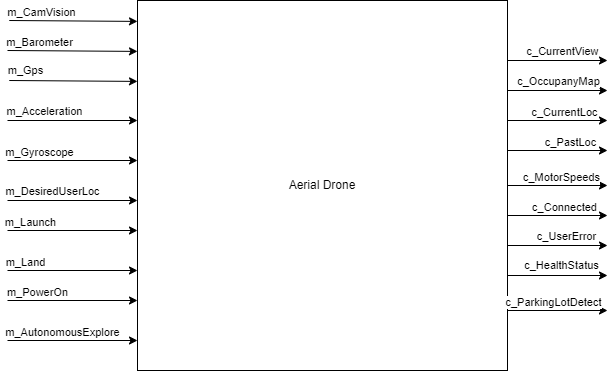
\includegraphics[width=0.5\textwidth]{ContextDiagram.png}
  \end{center}
\end{figure}



\begin{table}[!h]
\begin{center}
\caption {Input Variables} \label{tab:title}
\label{InputVariables}
\begin{tabular}{ | m{3cm} | m{2cm} | m{2cm} | m{6cm} | } 
\hline
 Variable Name & Type & Unit & Description \\ 
 \hline
 i\_MinHoverHeight & float	&m	& Minimum aerial hover height set by user\\
\hline i\_MaxHoverHeight & float	&m	& Maximum aerial hover height set by user\\
\hline i\_DesiredHoverHeight & float	&m	& Desired aerial hover height set by user\\
\hline 
\end{tabular}
\end{center}
\end{table}

\newpage
Monitored Variables are variables that are continuously monitored by the product.
\begin{table}[!h]
\begin{center}
\caption {Monitored Variables} \label{tab:title}
\begin{tabular}{ | m{3cm} | m{2cm} | m{2cm} | m{6cm} | } 
\hline
 Variable Name & Type & Unit & Description \\ 
 \hline
m\_Acceleration	& Vector& m/s^2 & three-dimensional vector containing acceleration relative to frame of the drone. \\
\hline
m\_Gyroscope & Vector	&Rad &	 three-dimensional vector containing orientation relative to frame of the drone.\\
\hline
m\_Gps	& Tuple &	\{DMS, m\} &	 current GPS coordinates of the drone with height in the second tuple.\\
\hline
m\_Barometer	& Float&	atm	 &Altitude detection using atmospheric pressure measurement\\
\hline
m\_DesiredUserLoc &	GPS Location& DMS &	 Desired location of the aerial drone set by user.\\
\hline
m\_Arm &	Boolean	 &  - &	Indicates if the operator desires the drone to arm.  \\
\hline
m\_Configure &	Boolean	 &  - &	Indicates if the operator desires the drone to configure height parameters.  \\
\hline
m\_Takeoff &	Boolean	 &  - &	Indicates if the operator desires the drone to takeoff.  \\
\hline
m\_AutonomousExplore &	Boolean &	 -	 &Indicates if the operator desires the drone to autonomously explore the parking lot.\\ 
\hline
m\_AutonomousMove &	Boolean &	 -	 & Indicates if the operator desires the drone to go to a specific GPS location through the Autonomous Move State.\\ 
\hline
m\_CompulsiveMove &	Boolean &	 -	 &Indicates if the operator desires the drone to go to a specific GPS location through the Compulsive Move State.\\ 
\hline
m\_PowerOn&	Boolean  &	- &	Indicates if the operator desires the drone to be On or Off.\\
\hline
m\_BatteryCapacity&	Float  &	sec &	Estimated flight time in battery remaining. \\
\hline
m\_Land&Boolean&	-&	Indicates if the operator desires the drone to land.\\
\hline
m\_SaveOutput&Boolean&	-&	Opens a dialog to save the current images and maps files in a folder.\\
\hline
 m\_CamVision &	Image&	Array of Pixels&	Latest image of the section of the parking lot currently visible to the drone.\\
\hline

\end{tabular}
\end{center}
\end{table}

\newpage

Controlled Variables are variables that are outputted by the system. Some are visible to the operator on their application, while others help to indirectly accomplish functional requirements. 

\begin{table}[!h]
\begin{center}
\caption {Controlled Variables} \label{tab:title}
\begin{tabular}{ | m{3cm} | m{2cm} | m{2cm} | m{6cm} |}
\hline
 Variable Name & Type & Unit & Description \\ 
 \hline
 c\_CurrentView &	Image &	Array of Pixels &	Live visual display of parking lot section the drone's currently sees, as well as any further annotations and text.\\
 \hline
c\_OccupancyMap &	Image &	Array of Pixels &	Map of available parking spots based on the drone’s previous paths. \\
\hline
c\_CurrentLoc & 	Tuple&	\{DMS, m\} & GPS coordinates are stored at the first index, height is stored in the second index.	Estimated longitudinal coordinate, lateral coordinate and height of the drone.\\
\hline
c\_PastLoc&	Vector &	DMS  &	Trace of the drone's location in the past 60 seconds (vector of GPS locations).\\
\hline
c\_MotorSpeeds &Vector&	   rad/s^2 &	 n-dimensional vector containing the motor speeds of however many motors the drone chooses to use (2 for helicopter, 4 for quadcopter, 6 for hexcopter, etc.). The vector contains speeds of each motor clockwise from front of the drone.\\

\hline

c\_Connected & Boolean &	- &	Indicates if connection between the drone and the operator's application is established\\
\hline
c\_ParkingLotDetected&	Boolean &	-&	Indicated if a parking lot is detected in the c_CurrentView.\\
\hline
c\_UserError &	Enumeration &	0 - None,
1 - Desired_Location_Out_Of_Bounds,
2 - No_Lot_Detected&	Indicates if a command the user requested is not feasible.\\
\hline
c\_HealthStatus &	Enumeration &	0 - Healthy,
1 - Unhealthy&	Indicates if the drone's mechanical and electrical state allows it to safely fly.  For example if there is mechanical damage, the value should be Unhealthy.\\
\hline
c\_Logs &	List of Strings &	- &	Contains a list of past log messages.\\
\hline
\end{tabular}
\end{center}
\end{table}





\newpage

\subsection{Functional Requirements}
\label{sec:funcReqs}
The following requirements are required in order to achieve the product's functions, as stated in \nameref{subsec:ProdFunc}.

\subsubsection{General Functional Requirements}

\begin{table}[!h]
\begin{center}
\caption {GEN\_001} 
\label{GEN_001}
\begin{tabular}{ | m{3cm} | m{11cm} | }
\hline
Description & The product shall be able to recognize Clear Boundaries \ref{DefTable}. This requirement is a refinement of the \nameref{Autonomous Explore State}. \\
\hline
Rationale & This requirement ensures that the product is able to implement basic autonomy, such as not traveling past the parking lot boundaries. \\
\hline
Phase & II \\
\hline
Likely to Change & No. This requirement is required to implement the \nameref{Autonomous Explore State}. \\
\hline
Associated Inputs and Outputs & m\_CamVision. \\
\hline
\end{tabular}
\end{center}
\end{table}


\begin{table}[!h]
\begin{center}
\caption {GEN\_002} 
\label{GEN_002}
\begin{tabular}{ | m{3cm} | m{11cm} | } 
\hline
Description & The product shall provide live update of c\_CurrentLoc, c\_CurrentView and c\_OccupancyMap during all normal and non-configurational operation states. This requirement is a refinement of the normal and non-configuration operation states specified in Section \ref{subsec:ProdFunc}. \\
\hline
Rationale & This requirement ensures that the product always provides the latest controlled variable information to the operator. \\
\hline
Phase & II \\
\hline
Likely to Change & No. This requirement is a part of the MVP and must be present to make the product achieve its product functions. \\
\hline
Associated Inputs and Outputs & m\_CamVision, c\_CurrentLoc, c\_CurrentView, and c\_OccupancyMap. \\
\hline
\end{tabular}
\end{center}
\end{table}

\begin{table}[!h]
\begin{center}
\caption {GEN\_003} 
\label{GEN_003}
\begin{tabular}{ | m{3cm} | m{11cm} | } 
\hline
Description & The product shall allow the operator to configure the i\_MinHoverHeight, i\_MaxHoverHeight, and i\_DesiredHoverHeight. This requirement is a refinement of the \nameref{Configure State}. \\
\hline
Rationale & The value of these parameters depends on the operators view preferences and parking lot conditions. For example a parking lot with a lot of large trucks may be better suited to higher hovering heights. \\
\hline
Phase & I \\
\hline
Likely to Change & No. This requirement is vital to the operation of the product, as it must be suited to different parking lot environments. \\
\hline
Associated Inputs and Outputs & i\_MinHoverHeight, i\_MaxHoverHeight, and i\_DesiredHoverHeight. \\
\hline
\end{tabular}
\end{center}
\end{table}

\begin{table}[!h]
\begin{center}
\caption {GEN\_004} 
\label{GEN_004}
\begin{tabular}{ | m{3cm} | m{11cm} | } 
\hline
Description & The condition i\_MinHoverHeight <= i\_DesiredHoverHeight <= i\_MaxHoverHeight shall always be true. This requirement is a refinement of the \nameref{Configure State}. \\
\hline
Rationale & This requirement ensures logical values for the parameters are set by the operator. \\
\hline
Phase & I \\
\hline
Likely to Change & No. This requirement is required to check the inputted values by the operator. \\
\hline
Associated Inputs and Outputs & i\_MinHoverHeight, i\_DesiredHoverHeight, and i\_MaxHoverHeight. \\
\hline
\end{tabular}
\end{center}
\end{table}

\begin{table}[!h]
\begin{center}
\caption {GEN\_005} 
\label{GEN_005}
\begin{tabular}{ | m{3cm} | m{11cm} |}
\hline
Description & The product shall be able to identify non-occupied parking spots. This requirement is a refinement of the normal and non-configuration operation states specified in Section \ref{subsec:ProdFunc}. \\
\hline
Rationale & This requirement ensures that the product is able to create the occupancy map. \\
\hline
Phase & III \\
\hline
Likely to Change & No. This requirement is required to create the occupancy map (c_OccupancyMap), which is one of the main functions of the product during the Phase III Release. \\
\hline
Associated Inputs and Outputs & m\_CamVision, c\_ParkingLotDetected, and c\_OccupancyMap. \\
\hline
\end{tabular}
\end{center}
\end{table}

\begin{table}[!h]
\begin{center}
\caption {GEN\_006} 
\label{GEN_006}
\begin{tabular}{ | m{3cm} | m{11cm} | }
\hline
Description & The product shall be shall highlight non-occupied parking slots on the operator's display (update c_CurrentView). This requirement is a refinement of the normal and non-configuration operation states specified in Section \ref{subsec:ProdFunc}. \\
\hline
Rationale & This requirement ensures that the product is able to create the occupancy map. \\
\hline
Phase & III \\
\hline
Likely to Change & No. This requirement is a key feature of the occupancy map in order to efficiently communicate the data to the operator. \\
\hline
Associated Inputs and Outputs & m\_CamVision, c\_CurrentView, c\_ParkingLotDetected, and c\_OccupancyMap. \\
\hline
\end{tabular}
\end{center}
\end{table}

\clearpage
\newpage

\subsubsection{State Implementation Requirements}
\label{sec:stateReqs}

\begin{table}[!h]
\begin{center}
\caption {STA\_000} 
\label{STA_000}
\begin{tabular}{ | m{3cm} | m{11cm} | } 

\hline
Description & The product shall implement an Idle state. During this state, the solution is powered on but motors are stationary. This requirement is a refinement of the \nameref{Idle State}, and further refined by \nameref{PERF_007}, \nameref{SAFE_001}, \nameref{SAFE_003}, and \nameref{USE_003}. \\
\hline
Rationale & This state is used to ensure that the operator can safely hold the drone and access the mechanical switch that controls m\_PowerOn. \\
\hline
Phase & I \\
\hline
Likely to Change & No. This requirement is required for the safety of the operator. \\
\hline
Associated Inputs and Outputs & m\_PowerOn and c\_Connected. \\
\hline
\end{tabular}
\end{center}
\end{table}

\begin{table}[!h]
\begin{center}
\caption {STA\_001} 
\label{STA_001}
\begin{tabular}{ | m{3cm} | m{11cm} | }
\hline
Description & The product shall implement a Hover State. During this state, the solution shall fly to and hover at a height of i\_MaxHoverHeight. The drone shall keep the same lateral location it is currently at. The drone cannot transition to another flight state until it has reached a height of i\_MaxHoverHeight. This requirement is a refinement of the \nameref{Hover State} and is further refined by \nameref{PERF_002}, \nameref{PERF_004}, \nameref{PERF_005}, \nameref{PERF_006}, \nameref{PERF_007}, \nameref{SAFE_001}, \nameref{SAFE_003}, and \nameref{USE_003}. \\
\hline
Rationale & This state is used for when the product is waiting for further operator commands. Hover height is selected to be i\_MaxHoverHeight, so that the drone can see as much of the parking lot section as it can. This makes the transition to \nameref{Autonomous Explore State} more likely.
The drone cannot exit the Hover state until it reaches i\_MaxHoverHeight. This feature is added to ensure that the drone moves does not move laterally until it has sufficient height. during this state. For example, if the drone is just launching from the ground, it is unsafe for the drone to transition to the \nameref{Autonomous Explore State} and move laterally (as it could collide with an object).    \\
\hline
Phase & II \\
\hline
Likely to Change & No. This requirement is a key feature of the MVP, and is required in order to gather any useful information to the operator. \\
\hline
Associated Inputs and Outputs & m\_Barometer, m\_Acceleration, m\_Gyroscope, m\_Gps, i\_MaxHoverHeight, and c\_MotorSpeeds. \\
\hline
\end{tabular}
\end{center}
\end{table}

\begin{table}[!h]
\begin{center}
\caption {STA\_002} 
\label{STA_002}
\begin{tabular}{ | m{3cm} | m{11cm} | }
\hline
Description & The product shall implement an Autonomous Move State. During this state, the drone moves to the m\_DesiredUserLoc if it is within the parking lot, and hovers at that location with height i\_DesiredHoverHeight. This requirement is a refinement of the \nameref{Autonomous Move State} and is further refined by \nameref{PERF_003}, \nameref{PERF_004}, \nameref{PERF_006}, \nameref{PERF_007}, \nameref{SAFE_001}, \nameref{SAFE_003}, \nameref{USE_003}, and \nameref{PERF_008}. \\
\hline
Rationale & This state is used for when the product needs to provide the operator the ability to move the drone to a specific location, with the functionality of stopping motion if the location is invalid. \\
\hline
Phase & II \\
\hline
Likely to Change & No. This requirement is a key feature of the product, and is required in order for the operator to make changes to the product's path. \\
\hline
Associated Inputs and Outputs & m\_DesiredUserLoc, m\_Barometer, m\_Acceleration, m\_Gyroscope, m\_Gps, i\_DesiredHoverHeight, and c\_MotorSpeeds. \\
\hline
\end{tabular}
\end{center}
\end{table}

\begin{table}[!h]
\begin{center}
\caption {STA\_003} 
\label{STA_003}
\begin{tabular}{ | m{3cm} | m{11cm} | }
\hline
Description & The product shall implement an Autonomous Explore State. During this state the drone will create its own path to explore and remain within the parking lot it currently detects. This requirement is a refinement of the \nameref{Autonomous Explore State} and is further refined by \nameref{PERF_001}, \nameref{PERF_004}, \nameref{PERF_007}, \nameref{SAFE_001}, \nameref{SAFE_003}, and \nameref{USE_003}. \\
\hline
Rationale & This state is used for when the operator does not need to constantly instruct the drone to move. \\
\hline
Phase & III \\
\hline
Likely to Change & No. This requirement is an important part of the Phase III Release, as it allows for automated creation of the occupancy map. \\
\hline
Associated Inputs and Outputs & m\_Barometer, m\_Acceleration, m\_Gyroscope, m\_Gps, m\_AutonomouseExplore, m\_CamVision, c\_CurrentView, and c\_MotorSpeeds. \\
\hline
\end{tabular}
\end{center}
\end{table}

\begin{table}[!h]
\begin{center}
\caption {STA\_004} 
\label{STA_004}
\begin{tabular}{ | m{3cm} | m{11cm} | }
\hline
Description & The product shall implement a Configure state. During this state settings and parameters that cannot be changed during flight can be changed. The Input Variables i\_MinHoverHeight, i\_MaxHoverHeight and i\_DesiredHoverHeight can be changed in this state. The product is powered on but motors are stationary. This requirement is a refinement of the \nameref{Configure State}, and references \nameref{GEN_003}. This is further refined by \nameref{PERF_004}, \nameref{PERF_007}, \nameref{SAFE_001}, \nameref{SAFE_003}, and \nameref{USE_003}. \\
\hline
Rationale & This state is used to allow parameters that are unsafe to change during flight operation, to be safely changed through a special process. During this state the operator can safely hold the drone. Such parameters are outlined in \nameref{InputVariables}. \\
\hline
Phase & II \\
\hline
Likely to Change & No. This requirement is required to ensure safety of the operator, as well as the product from unsafe changes during operation. \\
\hline
Associated Inputs and Outputs &  i\_MinHoverHeight, i\_MaxHoverHeight, and i\_DesiredHoverHeight. \\
\hline
\end{tabular}
\end{center}
\end{table}

\begin{table}[!h]
\begin{center}
\caption {STA\_005} 
\label{STA_005}
\begin{tabular}{ | m{3cm} | m{11cm} | }
\hline
Description & The product shall implement an Off state.  All modules are powered off. No battery power is consumer. c\_UserError is set to None, c\_HealthStatus is set to Healthy, and c\_Connected is set to false. All values in the matrices c\_MotorSpeeds, c\PastLoc, c\_OccupancyMap, and c\_CurrentView are set to 0. This requirement is a refinement of the \nameref{Off State} and is further refined by \nameref{PERF_004}, \nameref{PERF_007}, \nameref{SAFE_001}, and \nameref{SAFE_003} \\
\hline
Rationale & This state is used to explicitly state what it means for the drone to be off. \\
\hline
Phase & I \\
\hline
Likely to Change & No. This requirement is required for the safe operation, transport, and handling of the product. \\
\hline
Associated Inputs and Outputs & c\_UserError, c\_HealthStatus, c\_Connected, c\_MotorSpeeds, c\PastLoc, c\_OccupancyMap, and c\_CurrentView. \\
\hline
\end{tabular}
\end{center}
\end{table}

\begin{table}[!h]
\begin{center}
\caption {STA\_006} 
\label{STA_006}
\begin{tabular}{ | m{3cm} | m{11cm} | }
\hline
Description & The product shall implement a Land state. In the land state the solution first travel laterally to the initial launch location, and then lands vertically downward. After landing the drone enters the disarms and enters the Idle state. This requirement is a refinement of the \nameref{Land State} and is further refined by \nameref{PERF_002}, \nameref{PERF_004}, \nameref{PERF_006}, \nameref{PERF_007}, \nameref{SAFE_001}, \nameref{SAFE_003}, and \nameref{USE_003}. \\
\hline
Rationale & This state is used to explicitly designate a landing path and command. \\
\hline
Phase & II \\
\hline
Likely to Change & No. This requirement is required for stopping the operation of the product. \\
\hline
Associated Inputs and Outputs & m\_Barometer, m\_Acceleration, m\_Gyroscope, m\_Gps, and c\_MotorSpeeds. \\
\hline
\end{tabular}
\end{center}
\end{table}

\begin{table}[!h]
\begin{center}
\caption {STA\_007} 
\label{STA_007}
\begin{tabular}{ | m{3cm} | m{11cm} | }
\hline
Description & The product shall implement a Desired Location Error state. Upon entry to this state, the c\_UserError variable is set to Desired_Location_Out_Of_Bounds, and set to None upon exit. The drone proceeds to Hover at its current location. Upon exit of this state, the drone shall set c\_UserError to None. Upon entry, the message "Desired Location out of parking lot bounds" shall be logged into c\_Logs. This requirement is a refinement of the \nameref{Desired Location Error State} and is further refined by \nameref{PERF_007}, \nameref{SAFE_001}, \nameref{SAFE_003}, and \nameref{USE_003}. \\
\hline
Rationale & This state is used to indicate explicitly that the operator's request cannot be met.  \\
\hline
Phase & II \\
\hline
Likely to Change & No. This requirement is required for clear communication with the operator to handle unsupported requests. \\
\hline
Associated Inputs and Outputs & m\_Barometer, m\_Acceleration, m\_Gyroscope, m\_Gps, c\_UserError, c\_Logs and c\_MotorSpeeds. \\
\hline
\end{tabular}
\end{center}
\end{table}

\begin{table}[!h]
\begin{center}
\caption {STA\_008} 
\label{STA_008}
\begin{tabular}{ | m{3cm} | m{11cm} | }
\hline
Description & The product shall implement a No Parking Lot Detected Error state. Upon entry to this state, the c\_UserError variable is set to No_Lot_Detected_State, and while upon exit c\_UserError is set to None upon exit. The drone proceeds to Hover at its current location. Upon exit of this state, the drone shall set c\_UserError to None. Upon entry, the message "No Parking Lot detected." shall be logged into c\_Logs. This requirement is a refinement of the \nameref{No Parking Lot Detected Error State} and is further refined by \nameref{PERF_007}, \nameref{SAFE_001}, \nameref{SAFE_003}, and \nameref{USE_003}. \\
\hline
Rationale & This state is used to indicate explicitly that the product cannot detect a parking lot. \\
\hline
Phase & II \\
\hline
Likely to Change & No. This requirement is required for clear communication with the operator to handle unsupported requests. \\
\hline
Associated Inputs and Outputs & m\_Barometer, m\_Acceleration, m\_Gyroscope, m\_Gps, c\_UserError, c\_Logs, and c\_MotorSpeeds. \\
\hline
\end{tabular}
\end{center}
\end{table}

\begin{table}[!h]
\begin{center}
\caption {STA\_009} 
\label{STA_009}
\begin{tabular}{ | m{3cm} | m{11cm} | }
\hline
Description & The product shall implement a Malfunction state. Upon entry, the message "Major malfunction in drone detected, please inspect" shall be added to c\_Logs. During this state the drone sets the c\_HealthStatus to Unhealthy and sets c\_HealthStatus to Healthy upon exit. It then tries to land the product at its launch location, which if is not possible the drone instead lands vertically on the land below. After landing the drone enters the disarms and enters the Idle state. This requirement is a refinement of the \nameref{Malfunction State} and is further refined by \nameref{PERF_007}, \nameref{SAFE_001}, \nameref{SAFE_003}, and \nameref{USE_003}. \\
\hline
Rationale & This state is used to ensure that the product can handle large malfunctions that can occur during operation. \\
\hline
Phase & II \\
\hline
Likely to Change & No. This requirement is required to handle malfunctioning components during operation. \\
\hline
Associated Inputs and Outputs & m\_barometer, m\_acceleration, m\_gyroscope, m\_gps, c\_healthStatus, c\_Logs, and c\_motorSpeed. \\
\hline
\end{tabular}
\end{center}
\end{table}

\begin{table}[!h]
\begin{center}
\caption {STA\_010} 
\label{STA_010}
\begin{tabular}{ | m{3cm} | m{11cm} | }
\hline
Description & The product shall implement a Communication Lost state. During this state, the drone sets the c\_HealthStatus to Unhealthy, and a message "Connection with drone lost." is sent to the Operator's Application. Upon exit, "Connection with drone established." is logged to c\_Logs and c\_HealthStatus to Healthy. While in this state, the product tries to land at its launch location. After landing the drone enters the disarms and enters the Idle state. This requirement is a refinement of the \nameref{Communication Lost State} and is further refined by \nameref{PERF_007}, \nameref{SAFE_001}, \nameref{SAFE_003}, and \nameref{USE_003}. \\
\hline
Rationale & This state is used to ensure that the product can handle large malfunctions that can occur during operation. \\
\hline
Phase & II \\
\hline
Likely to Change & No. This requirement is required to handle malfunctioning components during operation. \\
\hline
Associated Inputs and Outputs & m\_barometer, m\_acceleration, m\_gyroscope, m\_gps, c\_healthStatus, and c\_motorSpeed. \\
\hline
\end{tabular}
\end{center}
\end{table}

\clearpage
\newpage

\begin{table}[!h]
\begin{center}
\caption {STA\_011} 
\label{STA_011}
\begin{tabular}{ | m{3cm} | m{11cm} | }
\hline
Description & The product shall implement a Compulsive Move State. During this state, the drone moves to the m\_DesiredUserLoc regardless of if it is within the parking lot, and hovers at that location with height i\_DesiredHoverHeight. This requirement is a refinement of the \nameref{Compulsive Move State} and is further refined by \nameref{PERF_003}, \nameref{PERF_004}, \nameref{PERF_006}, \nameref{PERF_007}, \nameref{SAFE_001}, \nameref{SAFE_003}, \nameref{PERF_008} and \nameref{USE_003}. \\
\hline
Rationale & This state is used for when the the product needs to provide the operator the ability to move the drone to a specific location. \\
\hline
Phase & II \\
\hline
Likely to Change & No. This requirement is a key feature of the product, and is required in order for the operator to make changes to the product's path. \\
\hline
Associated Inputs and Outputs & m\_DesiredUserLoc, m\_Barometer, m\_Acceleration, m\_Gyroscope, m\_Gps, i\_DesiredHoverHeight, and c\_MotorSpeeds. \\
\hline
\end{tabular}
\end{center}
\end{table}


\begin{table}[!h]
\begin{center}
\caption {STA\_012} 
\label{STA_012}
\begin{tabular}{ | m{3cm} | m{11cm} | }
\hline
Description & The product shall implement an Arm state. During this state, the drone attempts to arm the motor. Arming is essentially having the all motors spin, but not spin fast enough to generate liftoff. This requirement is a refinement of the \nameref{Arm State} and is further refined by \nameref{PERF_007}, \nameref{SAFE_001}, \nameref{SAFE_003}, and \nameref{USE_003}. \\
\hline
Rationale & This state is used to ensure that the product can handle large malfunctions that can occur during operation. \\
\hline
Phase & II \\
\hline
Likely to Change & No. This requirement is required to handle malfunctioning components during operation. \\
\hline
Associated Inputs and Outputs & m\_barometer, m\_acceleration, m\_gyroscope, m\_gps, c\_healthStatus, and c\_motorSpeed. \\
\hline
\end{tabular}
\end{center}
\end{table}

\begin{table}[!h]
\begin{center}
\caption {STA\_013} 
\label{STA_013}
\begin{tabular}{ | m{3cm} | m{11cm} | }
\hline
Description & The product shall implement a Takeoff state. During this state, the drone attempts to takeoff to i\_MaxHoverHeight. Arming is essentially having the all motors spin, but not spin fast enough to generate liftoff. This requirement is a refinement of the \nameref{Takeoff State} and is further refined by \nameref{PERF_002}, \nameref{PERF_007}, \nameref{SAFE_001}, \nameref{SAFE_003}, and \nameref{USE_003}. \\
\hline
Rationale & This state is used to ensure that the product can handle large malfunctions that can occur during operation. \\
\hline
Phase & II \\
\hline
Likely to Change & No. This requirement is required to handle malfunctioning components during operation. \\
\hline
Associated Inputs and Outputs & m\_barometer, m\_acceleration, m\_gyroscope, m\_gps, c\_healthStatus, and c\_motorSpeed. \\
\hline
\end{tabular}
\end{center}
\end{table}

\subsubsection{State Transition Requirements}
\label{transReqs}
The following requirements are refinements of all the states specified in Section \ref{sec:stateReqs}, and specifies the product's transitions between states. These requirements will not be changed unless the states are changed.

\begin{table}[!h]
\begin{center}
\caption {TRANS\_001} 
\label{TRANS_001}
\begin{tabular}{ | m{3cm} | m{11cm} | }
\hline
Description & Upon the m\_PowerOn becoming false, the drone shall enter the Off state. This requirement references the \nameref{Off State}. \\
\hline
Rationale & This requirement ensures that the product can turn off safely. \\
\hline
Phase & I \\
\hline
Associated Inputs and Outputs & m\_PowerOn. \\
\hline
\end{tabular}
\end{center}
\end{table}

\begin{table}[!h]
\begin{center}
\caption {TRANS\_002} 
\label{TRANS_002}
\begin{tabular}{ | m{3cm} | m{11cm} | }
\hline
Description & While in the \nameref{Off State}, upon the m\_PowerOn becoming true, the drone shall enter the Idle state. This requirement references the \nameref{Idle State} and the requirement \nameref{SAFE_005}. \\
\hline
Rationale & This requirement ensures that the propellers do not damage the operator after touching the m\_PowerOn switch.  \\
\hline
Phase & I \\
\hline
Associated Inputs and Outputs & m\_PowerOn. \\
\hline
\end{tabular}
\end{center}
\end{table}

\begin{table}[!h]
\begin{center}
\caption {TRANS\_003} 
\label{TRANS_003}
\begin{tabular}{ | m{3cm} | m{11cm} | }
\hline
Description & While in the \nameref{Idle State}, upon the m\_Arm becoming true the drone shall enter the Arm state. And upon the m\_Configure the drone should enter the Configure state. This requirement references the \nameref{Arm State} and the \nameref{Configure State}. \\
\hline
Rationale & This requirement facilitates the setup and configuration of the product.  \\
\hline
Phase & II \\
\hline
Associated Inputs and Outputs & m\_Arm and m\_Configure. \\
\hline
\end{tabular}
\end{center}
\end{table}

\begin{table}[!h]
\begin{center}
\caption {TRANS\_004} 
\label{TRANS_004}
\begin{tabular}{ | m{3cm} | m{11cm} | }
\hline
Description & If in the Hover state, and c\_ParkingLotDetected is equal to true, the product shall enter the Autonomous Explore state and explore the detected lot. If two parking lots are detected at the same time, it arbitrarily picks one to explore. This requirement references the \nameref{Hover State} and the \nameref{Autonomous Explore State}. \\
\hline
Rationale & This requirement ensures that the default mode of operation is Autonomous Explore after entering the Hover state.  \\
\hline
Phase & III \\
\hline
Associated Inputs and Outputs & c\_ParkingLotDetected. \\
\hline
\end{tabular}
\end{center}
\end{table}

\begin{table}[!h]
\begin{center}
\caption {TRANS\_005} 
\label{TRANS_005}
\begin{tabular}{ | m{3cm} | m{11cm} | }
\hline
Description & Upon m\_AutonomousMove is asserted to true, the drone shall automatically enter the Autonomous Move state. This requirement references the \nameref{Autonomous Move State}. \\
\hline
Rationale & This requirement ensures that the product shall take the operator's request with higher priority than any other kind of operation. \\
\hline
Phase & II \\
\hline
Associated Inputs and Outputs & m\_DesiredUserLoc, m\_CompulsiveMove. \\
\hline
\end{tabular}
\end{center}
\end{table}

\begin{table}[!h]
\begin{center}
\caption {TRANS\_006} 
\label{TRANS_006}
\begin{tabular}{ | m{3cm} | m{11cm} | }
\hline
Description & If while in the Autonomous Move State and the product determines that m\_DesiredUserLoc is outside parking lot boundaries, the product shall enter the Desired Location Error state. This requirement references the \nameref{Autonomous Move State} and the \nameref{Desired Location Error State}. \\
\hline
Rationale & This requirement ensures that the product shall notify any issues with the operator's request at the moment it is detected, so that the operator can make adjustments. \\
\hline
Phase & II \\
\hline
Associated Inputs and Outputs & m\_DesiredUserLoc. \\
\hline
\end{tabular}
\end{center}
\end{table}

\begin{table}[!h]
\begin{center}
\caption {TRANS\_007} 
\label{TRANS_007}
\begin{tabular}{ | m{3cm} | m{11cm} | }
\hline
Description & When m\_AutonomousExplore is set to true and c\_ParkingLotDetected is equal to true, the product shall enter the Autonomous Explore state. This requirement references the \nameref{Autonomous Explore State}. \\
\hline
Rationale & This requirement ensures that the product shall take the operator's request with higher priority than any other kind of operation. \\
\hline
Phase & II \\
\hline
Associated Inputs and Outputs & m\_AutonomousExplore and c\_ParkingLotDetected. \\
\hline
\end{tabular}
\end{center}
\end{table}

\begin{table}[!h]
\begin{center}
\caption {TRANS\_008} 
\label{TRANS_008}
\begin{tabular}{ | m{3cm} | m{11cm} | }
\hline
Description & When m\_AutonomousExplore is set to true but c\_ParkingLotDetected is equal to false, the product shall enter the No Parking Lot Detected Error state. This requirement references the \nameref{No Parking Lot Detected Error State}. \\
\hline
Rationale & This requirement ensures that the product shall notify any issues with the operator's request at the moment it is detected, so that the operator can make adjustments. \\
\hline
Phase & II \\
\hline
Associated Inputs and Outputs & m\_AutonomousExplore and c\_ParkingLotDetected. \\
\hline
\end{tabular}
\end{center}
\end{table}

\begin{table}[!h]
\begin{center}
\caption {TRANS\_009} 
\label{TRANS_009}
\begin{tabular}{ | m{3cm} | m{11cm} | }
\hline
Description & Upon m\_Land being true, the product shall enter the Land state. This requirement references the \nameref{Land State}. \\
\hline
Rationale & This requirement ensures that the product is able to land at the requested time. \\
\hline
Phase & II \\
\hline
Associated Inputs and Outputs & m\_Land. \\
\hline
\end{tabular}
\end{center}
\end{table}

\begin{table}[!h]
\begin{center}
\caption {TRANS\_010} 
\label{TRANS_010}
\begin{tabular}{ | m{3cm} | m{11cm} | }
\hline
Description & If c\_Connected becomes false for more than 5 seconds, or signal strength (dBm) has lost 80\% of its typical value at any point during operation, then the product shall enter the Communication Lost state. This requirement references the \nameref{Communication Lost State}. \\
\hline
Rationale & This requirement ensures that the product detects connectivity errors, and is able to handle such occurrences. \\
\hline
Phase & I \\
\hline
Associated Inputs and Outputs & c\_Connected. \\
\hline
\end{tabular}
\end{center}
\end{table}

\begin{table}[!h]
\begin{center}
\caption {TRANS\_011} 
\label{TRANS_011}
\begin{tabular}{ | m{3cm} | m{11cm} | }
\hline
Description & If while in the Communication Lost State, c\_Connected becomes true for more than 5 seconds, or signal strength (dBm) has returned to 50\% of its typical value at any point during operation, then the product shall enter the Hover state. This requirement references the \nameref{Communication Lost State}. \\
\hline
Rationale & This requirement ensures that the product resumes normal operation once connectivity is regained. \\
\hline
Phase & I \\
\hline
Associated Inputs and Outputs & c\_Connected. \\
\hline
\end{tabular}
\end{center}
\end{table}

\begin{table}[!h]
\begin{center}
\caption {TRANS\_012} 
\label{TRANS_012}
\begin{tabular}{ | m{3cm} | m{11cm} | }
\hline
Description & Upon the user asserting m\_CompulsiveMove is as true, the drone shall automatically enter the Compulsive Move state. This requirement references the \nameref{Compulsive Move State}. \\
\hline
Rationale & This requirement ensures that the product shall take the operator's request with higher priority than any other kind of operation. \\
\hline
Phase & II \\
\hline
Associated Inputs and Outputs & m\_DesiredUserLoc, m\_CompulsiveMove. \\
\hline
\end{tabular}
\end{center}
\end{table}

\begin{table}[!h]
\begin{center}
\caption {TRANS\_013} 
\label{TRANS_013}
\begin{tabular}{ | m{3cm} | m{11cm} | }
\hline
Description & While in the \nameref{Arm State}, upon the m\_Takeoff becoming true the drone shall enter the Arm state. This requirement references the \nameref{Arm State} and the \nameref{Takeoff State}. \\
\hline
Rationale & This requirement facilitates breaking up the launching process so that if there are any issues they can be detected early.  \\
\hline
Phase & II \\
\hline
Associated Inputs and Outputs & m\_Takeoff. \\
\hline
\end{tabular}
\end{center}
\end{table}

\begin{table}[!h]
\begin{center}
\caption {TRANS\_014} 
\label{TRANS_014}
\begin{tabular}{ | m{3cm} | m{11cm} | }
\hline
Description & While in the \nameref{Takeoff State}, upon the drone reaching within 1 meter of i\_MaxHoverHeight, the drone should transition to the \nameref{Hover State}. This requirement references the \nameref{Hover State} and the \nameref{Takeoff State}. \\
\hline
Rationale & This requirement facilitates the setup and configuration of the product.  \\
\hline
Phase & II \\
\hline
Associated Inputs and Outputs & m\_Barometer. \\
\hline
\end{tabular}
\end{center}
\end{table}

\begin{table}[!h]
\begin{center}
\caption {TRANS\_015} 
\label{TRANS_015}
\begin{tabular}{ | m{3cm} | m{11cm} | }
\hline
Description & While in the \nameref{Configure State}, once the height parameters have been updated, the drone should transition back to the \nameref{Idle State}. This requirement references the \nameref{Configure State} and the \nameref{Idle State}. \\
\hline
Rationale & This requirement facilitates the setup and configuration of the product.  \\
\hline
Phase & II \\
\hline
Associated Inputs and Outputs & \\
\hline
\end{tabular}
\end{center}
\end{table}

\begin{table}[!h]
\begin{center}
\caption {A tractability table linking non-functional requirements to the functional requirements they reference. If a requirement has no dependencies or relationships, then it is not mentioned. }
\label{TRACE_FR_NFR}
\begin{tabular}{ | m{7cm} | m{7cm} | }
\hline
Functional Requirement & Non-functional requirement  \\
\hline
\nameref{STA_000} & \nameref{PERF_007}, \nameref{SAFE_001}, \nameref{SAFE_003}, \nameref{USE_003}  \\
\hline
\nameref{STA_001} & \nameref{PERF_002}, \nameref{PERF_004}, \nameref{PERF_005}, \nameref{PERF_006}, \nameref{PERF_007}, \nameref{SAFE_001}, \nameref{SAFE_003}, \nameref{USE_003}  \\
\hline
\nameref{STA_002} & \nameref{PERF_003}, \nameref{PERF_004}, \nameref{PERF_006}, \nameref{PERF_007}, \nameref{SAFE_001}, \nameref{SAFE_003}, \nameref{USE_003}  \\
\hline
\nameref{STA_003} & \nameref{PERF_001}, \nameref{PERF_004}, \nameref{PERF_007}, \nameref{SAFE_001}, \nameref{SAFE_003}, \nameref{USE_003}  \\
\hline
\nameref{STA_004} & \nameref{PERF_004}, \nameref{PERF_007}, \nameref{SAFE_001}, \nameref{SAFE_003}, \nameref{USE_003}  \\
\hline
\nameref{STA_005} & \nameref{PERF_004}, \nameref{PERF_007}, \nameref{SAFE_001}, \nameref{SAFE_003}  \\
\hline
\nameref{STA_006} & \nameref{PERF_002}, \nameref{PERF_004}, \nameref{PERF_006}, \nameref{PERF_007}, \nameref{SAFE_001}, \nameref{SAFE_003}, \nameref{USE_003}  \\
\hline
\nameref{STA_007} & \nameref{PERF_007}, \nameref{SAFE_001}, \nameref{SAFE_003}, \nameref{USE_003}  \\
\hline
\nameref{STA_008} & \nameref{PERF_007}, \nameref{SAFE_001}, \nameref{SAFE_003}, \nameref{USE_003}  \\
\hline
\nameref{STA_009} & \nameref{PERF_007}, \nameref{SAFE_001}, \nameref{SAFE_003}, \nameref{USE_003}  \\
\hline
\hline
\nameref{STA_010} & \nameref{PERF_007}, \nameref{SAFE_001}, \nameref{SAFE_003}, \nameref{USE_003}  \\
\hline
\nameref{STA_011} & \nameref{PERF_003}, \nameref{PERF_004}, \nameref{PERF_006}, \nameref{PERF_007}, \nameref{SAFE_001}, \nameref{SAFE_003}, \nameref{USE_003}  \\
\hline
\nameref{STA_012} & \nameref{PERF_007}, \nameref{SAFE_001}, \nameref{SAFE_003}, \nameref{USE_003}  \\
\hline
\nameref{STA_013} & \nameref{PERF_002}, \nameref{PERF_007}, \nameref{SAFE_001}, \nameref{SAFE_003}, \nameref{USE_003}  \\
\hline

\end{tabular}
\end{center}
\end{table}

\begin{table}[!h]
\begin{center}
\caption {A tracability table linking functional requirements to the functions they refine. If a requirement has no dependencies or relationships, then it is not mentioned. }
\label{TRACE_FR_Func}
\begin{tabular}{ | m{7cm} | m{7cm} | }
\hline
Functional Requirement & Function  \\
\hline
\nameref{GEN_001} & \nameref{Autonomous Explore State},\nameref{Autonomous Move State}  \\
\hline
\nameref{STA_000} & \nameref{Idle State}  \\
\hline
\nameref{STA_001} & \nameref{Hover State}  \\
\hline
\nameref{STA_002} & \nameref{Autonomous Move State}  \\
\hline
\nameref{STA_003} & \nameref{Autonomous Explore State}  \\
\hline
\nameref{STA_004} & \nameref{Configure State}  \\
\hline
\nameref{STA_005} & \nameref{Off State}  \\
\hline
\nameref{STA_006} & \nameref{Land State}  \\
\hline
\nameref{STA_007} & \nameref{Desired Location Error State}  \\
\hline
\nameref{STA_008} & \nameref{No Parking Lot Detected Error State}  \\
\hline
\nameref{STA_009} & \nameref{Malfunction State}  \\
\hline
\nameref{STA_010} & \nameref{Communication Lost State}  \\
\hline
\nameref{STA_011} & \nameref{Compulsive Move State}  \\
\hline
\end{tabular}
\end{center}
\end{table}

\clearpage
\newpage

\subsection{Performance Requirements}


\begin{table}[!h]
\begin{center}
\caption {PERF\_001} 
\label{PERF_001}
\begin{tabular}{ | m{3cm} | m{11cm} | }
\hline
Description & The product shall be capable of exploring upto 1400 $ m^2 $ of the detected parking lot during the \nameref{Autonomous Explore State}. This is a refinement of \nameref{STA_003}. \\
\hline
Rationale & The requirement ensures that \nameref{Autonomous Explore State} is able to survey atleast 60 parking spots each of size 13.5 $ m^2 $, assuming 6m of parking space between rows of parking. \\
\hline
Phase & III \\
\hline
Likely to Change & Yes. Based on algorithm performance of autonomous exploration and the limitations of the hardware, the threshold may be required to change. \\
\hline
Associated Inputs and Outputs & m\_barometer, m\_acceleration, m\_gyroscope, m\_gps, m\_AutonomousExplore, and c\_MotorSpeeds.  \\
\hline
\end{tabular}
\end{center}
\end{table}

\begin{table}[!h]
\begin{center}
\caption {PERF\_002} 
\label{PERF_002}
\begin{tabular}{ | m{3cm} | m{11cm} | }
\hline
Description & The product shall takeoff to i\_MaxHoverHeight and land from i\_MaxHoverHeight within 25 seconds. This requirement are refinements of \nameref{STA_001} and \nameref{STA_006}.  \\
\hline
Rationale &  The requirement ensures that minimal time is required for the product to start transmitting useful data to the operator, and that it does not take excessive time to cease operation once finished. \\
\hline
Phase & II \\
\hline
Likely to Change & No. This requirement refines the Minimum Viable Product and should not be modified. \\
\hline
Associated Inputs and Outputs & m\_barometer, m\_acceleration, m\_gyroscope, m\_gps, and c\_MotorSpeeds.  \\
\hline
\end{tabular}
\end{center}
\end{table}

\begin{table}[!h]
\begin{center}
\caption {PERF\_003} 
\label{PERF_003}
\begin{tabular}{ | m{3cm} | m{11cm} | }
\hline
Description & The product shall move to a specified location with an average speed exceeding 4km/hour. This is a refinement of \nameref{STA_002}. \\
\hline
Rationale & The requirement ensures that the operator spends minimal time waiting for the product to move to the desired location, and that it is quicker than the average speed of a person walking.  \\
\hline
Phase & II \\
\hline
Likely to Change & No. This requirement refines the movement of the product to ensure that the product is more optimal than a human. \\
\hline
Associated Inputs and Outputs & m\_barometer, m\_acceleration, m\_gyroscope, m\_gps, and c\_MotorSpeeds.  \\
\hline
\end{tabular}
\end{center}
\end{table}

\begin{table}[!h]
\begin{center}
\caption {PERF\_004} 
\label{PERF_004}
\begin{tabular}{ | m{3cm} | m{11cm} | }
\hline
Description & The product shall transmit all data to the operator at a rate exceeding 0.5 frames per second. This is a refinement of the functions specified in Section \nameref{subsec:ProdFunc}. \\
\hline
Rationale & The requirement ensures the operator is receiving real time data from the product. \\
\hline
Phase & I \\
\hline
Likely to Change & No. This requirement constitutes the MVP, and ensures that the operator is able to receive the information in a timely manner. \\
\hline
Associated Inputs and Outputs & m\_barometer, m\_acceleration, m\_gyroscope, m\_gps, m\_CamVision, c\_CurrentView, c\_CurrentLoc, c\_PastLoc, and c\_MotorSpeeds.  \\
\hline
\end{tabular}
\end{center}
\end{table}

\begin{table}[!h]
\begin{center}
\caption {PERF\_005} 
\label{PERF_005}
\begin{tabular}{ | m{3cm} | m{11cm} | }
\hline
Description & The product shall maintain a longitudinal and lateral position within a 1.5m radius during the \nameref{Hover State}. This requirement is a refinement of \nameref{STA_001}. \\
\hline
Rationale & The requirement ensures that the product does not drift to a different location when the operator expects it to be stationary. \\
\hline
Phase & II \\
\hline
Likely to Change & No. This requirement is required to allow proper operation of the product, as excessive drifting will cause inaccurate data to the operator. \\
\hline
Associated Inputs and Outputs & m\_barometer, m\_acceleration, m\_gyroscope, m\_gps, c\_CurrentLoc, and c\_MotorSpeeds.  \\
\hline
\end{tabular}
\end{center}
\end{table}

\begin{table}[!h]
\begin{center}
\caption {PERF\_006} 
\label{PERF_006}
\begin{tabular}{ | m{3cm} | m{11cm} | }
\hline
Description & While the product is in a flying state that is not Takeoff the drone shall always maintain an altitude between i\_MaxHoverHeight and i\_MinHoverHeight, within a tolerance of ±5\%. This requirement are refinements of \nameref{STA_001}, \nameref{STA_002}, \nameref{STA_011} and \nameref{STA_003}.  \\
\hline
Rationale & The requirement ensures that the operator specified altitude limits are respected during operation of the product. \\
\hline
Phase & II \\
\hline
Likely to Change & No. This requirement ensures that the operator's commands are respected during operation. \\
\hline
Associated Inputs and Outputs & m\_barometer, i\_MaxHoverHeight, i\_MinHoverHeight, and c\_MotorSpeeds.  \\
\hline
\end{tabular}
\end{center}
\end{table}

\begin{table}[!h]
\begin{center}
\caption {PERF\_007} 
\label{PERF_007}
\begin{tabular}{ | m{3cm} | m{11cm} | }
\hline
Description & The product shall be operable within requirements within non-inclement weather \ref{DefTable}.  This requirement are refinements of all the functions stated in Section \nameref{subsec:ProdFunc}, and the assumption of the weather in Section \nameref{sec:Assumptions}. This is further refined within requirement \nameref{MTNC_003}. \\
\hline
Rationale & The requirement ensures that the product is usable in the majority of the environmental conditions, such that its availability is maximized. \\
\hline
Phase & III \\
\hline
Likely to Change &  Yes. Based on hardware limitations, this requirement may need to be modified to include less adverse weather conditions.  \\
\hline
Associated Inputs and Outputs & m\_barometer, m\_acceleration, m\_gyroscope, m\_gps, c\_CurrentView, c\_CurrentLoc, c\PastLoc, and c\_MotorSpeeds.  \\
\hline
\end{tabular}
\end{center}
\end{table}

\begin{table}[!h]
\begin{center}
\caption {PERF\_008} 
\label{PERF_008}
\begin{tabular}{ | m{3cm} | m{11cm} | }
\hline
Description & The product shall maintain a longitudinal and lateral position within a 1.5m radius once the product has reached m\_DesiredUserLoc while in the \nameref{Autonomous Move State} or \nameref{Compulsive Move State}. This requirement is a refinement of \nameref{STA_002} and \nameref{STA_011}. \\
\hline
Rationale & The requirement ensures that the product does not drift to a different location when the operator expects it to be stationary. \\
\hline
Phase & II \\
\hline
Likely to Change & No. This requirement is required to allow proper operation of the product, as excessive drifting will cause inaccurate data to the operator. \\
\hline
Associated Inputs and Outputs & m\_barometer, m\_acceleration, m\_gyroscope, m\_gps, c\_CurrentLoc, and c\_MotorSpeeds.  \\
\hline
\end{tabular}
\end{center}
\end{table}

\clearpage
\newpage

\subsection{Logical Database Requirements}
There is no requirement for databases, as the problem requires no long-term storage of data.

\subsection{Design constraints }
\begin{table}[!h]
\begin{center}
\caption {DES\_001} 
\label{DES_001}
\begin{tabular}{ | m{3cm} | m{11cm} | }
\hline
Description & The product shall cost less than \$750 to manufacture. This requirement refines the constraint specified in Section \nameref{sec:Constraints}. \\
\hline
Rationale & The requirement ensures the constraint of the design is met, and ensures that it is not costly for users to implement or replace the product. \\
\hline
Phase & I \\
\hline
Likely to Change &  No. This requirement must be met in order to satisfy the externally imposed constraint. \\
\hline
Associated Inputs and Outputs & N/A.  \\
\hline
\end{tabular}
\end{center}
\end{table}

\subsection{Standards Compliance }
\begin{table}[!h]
\begin{center}
\caption {STD\_001} 
\label{STD_001}
\begin{tabular}{ | m{3cm} | m{11cm} | }
\hline
Description & The product shall weight a total of less than 25kg. This requirement refines the constraint specified in Section \nameref{sec:Constraints}. \\
\hline
Rationale & The requirement ensures the constraint of the design is met, and ensures that the product abides by Canadian regulatory laws. \\
\hline
Phase & I \\
\hline
Likely to Change &  No. This requirement must be met in order to satisfy the externally imposed constraint. \\
\hline
Associated Inputs and Outputs & N/A.  \\
\hline
\end{tabular}
\end{center}
\end{table}

\begin{table}[!h]
\begin{center}
\caption {STD\_002} 
\label{STD_002}
\begin{tabular}{ | m{3cm} | m{11cm} | }
\hline
Description & The product shall use radio communication only within the 2.4 GHz or 900 MHz range. This requirement refines the constraint specified in Section \nameref{sec:Constraints}. \\
\hline
Rationale & The requirement ensures the constraint of the design is met, and ensures that the product abides by Canadian regulatory laws. \\
\hline
Phase & I \\
\hline
Likely to Change &  No. This requirement must be met in order to satisfy the externally imposed constraint. \\
\hline
Associated Inputs and Outputs & N/A.  \\
\hline
\end{tabular}
\end{center}
\end{table}

\subsection{Software System Attributes}
There are no requirements regarding the software used in the product, provided that it meets all the other requirements specified within Section \ref{sec:Req}.

\subsection{Reliability }
There are no requirements for the reliability of the product, provided that it meets all the other requirements specified within Section \ref{sec:Req}.

\subsection{Availability}
There are no requirements for the reliability of the product, provided that it meets all the other requirements specified within Section \ref{sec:Req}.

\subsection{Security}
\begin{table}[!h]
\begin{center}
\caption {SEC\_001} 
\label{SEC_001}
\begin{tabular}{ | m{3cm} | m{11cm} | }
\hline
Description & The operator's application shall only be launched by a user with authorized access. \\
\hline
Rationale & The requirement ensures that non-authorized users cannot access the product's technology. \\
\hline
Phase & III \\
\hline
Likely to Change & Yes. This requirement may be modified or refined in future revisions of the product. \\
\hline
Associated Inputs and Outputs & N/A.  \\
\hline
\end{tabular}
\end{center}
\end{table}

\begin{table}[!h]
\begin{center}
\caption {SEC\_002} 
\label{SEC_002}
\begin{tabular}{ | m{3cm} | m{11cm} | }
\hline
Description & The product shall not upload any gathered data to any external parties. \\
\hline
Rationale & The requirement ensures the user's privacy and the event organizer's privacy. \\
\hline
Phase & II \\
\hline
Likely to Change & Yes. This requirement may be modified in future revisions if the need for off-board computation arises within the software. \\
\hline
Associated Inputs and Outputs & N/A.  \\
\hline
\end{tabular}
\end{center}
\end{table}

\clearpage
\newpage

\subsection{Maintainability}
\begin{table}[!h]
\begin{center}
\caption {MTNC\_001} 
\label{MTNC_001}
\begin{tabular}{ | m{3cm} | m{11cm} | }
\hline
Description & The product shall be fully recharged within 1 hour. This requirement references \nameref{USE_003}. \\
\hline
Rationale & The requirement ensures that the availability of the product is maximized, allowing for frequent uses of the product. \\
\hline
Phase & I \\
\hline
Likely to Change & Yes. This requirement may be limited by hardware requirements of the product. In later revisions, it may be modified to allow easy battery switching in the event that higher availability of the product is required. \\
\hline
Associated Inputs and Outputs & N/A.  \\
\hline
\end{tabular}
\end{center}
\end{table}

\begin{table}[!h]
\begin{center}
\caption {MTNC\_002} 
\label{MTNC_002}
\begin{tabular}{ | m{3cm} | m{11cm} | }
\hline
Description & The product shall be able to sustain a fall of greater than 1m without sustaining damage that affects operation performance. This requirement references the user classes of the product.\\
\hline
Rationale & The requirement ensures durability. Durability is important because the operators are not technical and may not know how to fix a broken product. \\
\hline
Phase & II \\
\hline
Likely to Change & Yes. This requirement may be limited by hardware requirements of the product. In later revisions, it may be modified to increase or decrease the fall height to better suit the available components. \\
\hline
Associated Inputs and Outputs & N/A.  \\
\hline
\end{tabular}
\end{center}
\end{table}

\begin{table}[!h]
\begin{center}
\caption {MTNC\_003} 
\label{MTNC_003}
\begin{tabular}{ | m{3cm} | m{11cm} | }
\hline
Description & The product shall be mechanically waterproof, to the point it can sustain a light drizzle for 1 minute of operation while still performing within the requirements. This requirement refines \nameref{PERF_007}. \\
\hline
Rationale & The requirement ensures that if the product experiences a drizzle during flight due to the operator incorrectly assuming the weather was dry, that the product is not severely damaged. \\
\hline
Phase & III \\
\hline
Likely to Change & Yes. This requirement may be limited by hardware requirements of the product. \\
\hline
Associated Inputs and Outputs & N/A.  \\
\hline
\end{tabular}
\end{center}
\end{table}

\clearpage
\newpage

\subsection{Safety}
\begin{table}[!h]
\begin{center}
\caption {SAFE\_001} 
\label{SAFE_001}
\begin{tabular}{ | m{3cm} | m{11cm} | }
\hline
Description & The product shall not influence or interact with dynamic actors positioned in the parking lot. This requirement is a refinement of the product functions stated within Section \nameref{subsec:ProdFunc}, and is further refined by \nameref{SAFE_002} and \nameref{SAFE_004}. \\
\hline
Rationale & The requirement ensures the product does not negatively impact the safety of visitors in the parking lot.  \\
\hline
Phase & I \\
\hline
Likely to Change & No. One of the fundamental product goals is to assist in parking lot traffic. If the product negatively impacts the traffic, there is no use in the product. \\
\hline
Associated Inputs and Outputs & N/A.  \\
\hline
\end{tabular}
\end{center}
\end{table}

\begin{table}[!h]
\begin{center}
\caption {SAFE\_002} 
\label{SAFE_002}
\begin{tabular}{ | m{3cm} | m{11cm} | }
\hline
Description & The product shall not allow the operator to set i\_MaxHoverHeight, i\_MinHoverHeight, or i\_DesiredHoverHeight to be below 7m. This requirement is a refinement of \nameref{SAFE_001}. \\
\hline
Rationale & The requirement ensures that the product does not interfere with existing traffic and that the flight path is above the majority of obstacles.  \\
\hline
Phase & I \\
\hline
Likely to Change & No. A selected height of below 7m drastically increases the amount of potential obstacles, which will further increase the complexity of the product. \\
\hline
Associated Inputs and Outputs & i\_MaxHoverHeight, i\_MinHoverHeight, and i\_DesiredHoverHeight.  \\
\hline
\end{tabular}
\end{center}
\end{table}

\begin{table}[!h]
\begin{center}
\caption {SAFE\_003} 
\label{SAFE_003}
\begin{tabular}{ | m{3cm} | m{11cm} | }
\hline
Description & The product shall not require the operator to physically manipulate the product in any way in any states outside of Off State. This requirement are further refinements of all the states outlined in Section \ref{subsec:ProdFunc}.  \\
\hline
Rationale & The requirement ensures that the operator does not interfere with the functions of the product, and that the operator is kept safe from any malfunctions of the product.  \\
\hline
Phase & I \\
\hline
Likely to Change & No. To maintain operator safety, the operator must never be required to be near the product during operation. This ensures that in the case of product failure, the operator is not harmed. \\
\hline
Associated Inputs and Outputs & N/A \\
\hline
\end{tabular}
\end{center}
\end{table}

\begin{table}[!h]
\begin{center}
\caption {SAFE\_004} 
\label{SAFE_004}
\begin{tabular}{ | m{3cm} | m{11cm} | }
\hline
Description & The product shall not cause distractions or negatively impact greater than 2\% of the visitors in the parking lot. This requirement is a refinement of \nameref{SAFE_001}. \\
\hline
Rationale & The requirement ensures that the usage of the product does not negatively impact the visitors in the parking lot.  \\
\hline
Phase & I \\
\hline
Likely to Change & No. One of the fundamental product goals is to assist in parking lot traffic. If the product negatively impacts the visitors, there is no use in the product. \\
\hline
Associated Inputs and Outputs & N/A \\
\hline
\end{tabular}
\end{center}
\end{table}

\begin{table}[!h]
\begin{center}
\caption {SAFE\_005} 
\label{SAFE_005}
\begin{tabular}{ | m{3cm} | m{11cm} | }
\hline
Description & The product shall include a mechanical Off switch to the product. This requirement is a refinement of the \nameref{Off State}.  \\
\hline
Rationale & The requirement ensures that the product can be turned off even in the case of electronic failures, and can double as a kill switch.  \\
\hline
Phase & I \\
\hline
Likely to Change & No. A kill switch independent from the electronics is essential to the safe operation of electromechanical products, and must be required within the product. \\
\hline
Associated Inputs and Outputs & N/A \\
\hline
\end{tabular}
\end{center}
\end{table}

\clearpage
\newpage

\subsection{Usability}
\begin{table}[!h]
\begin{center}
\caption {USE\_001} 
\label{USE_001}
\begin{tabular}{ | m{3cm} | m{11cm} | }
\hline
Description & The product shall provide a visual trace of its location for the past 60 seconds +- 1 second. This requirement is a refinement of the c\_CurrentView data. \\
\hline
Rationale & The requirement ensures that the operator is able to keep track of the product's past movement to understand which areas of the parking lot have been explored. \\
\hline
Phase & II \\
\hline
Likely to Change & Yes. Although a method of visualizing the past path is required, the method at which it is done may be changed in future revisions.  \\
\hline
Associated Inputs and Outputs & m\_barometer, m\_acceleration, m\_gyroscope, m\_gps, c\_CurrentView, c\_CurrentLoc, and c\_PastLoc.  \\
\hline
\end{tabular}
\end{center}
\end{table}

\begin{table}[!h]
\begin{center}
\caption {USE\_002} 
\label{USE_002}
\begin{tabular}{ | m{3cm} | m{11cm} | }
\hline
Description & Upon m\_SaveOutput becoming true, a file dialog shall open to let the operator save the current visual of c\_CurrentView and c\_OccupancyMap onto the operator's PC.  \\
\hline
Rationale & The requirement ensures that the operator can save the current data for future reference and analysis, and provides a digital record of its operation. \\
\hline
Phase & III \\
\hline
Likely to Change & Yes. The method of which the operator saves the data, or which data is saved, may  be changed in future revisions. \\
\hline
Associated Inputs and Outputs & m\_Barometer, m\_Acceleration, m\_Gyroscope, m\_gps, c\_CurrentView, c\_CurrentLoc, and c\_PastLoc.  \\
\hline
\end{tabular}
\end{center}
\end{table}

\begin{table}[!h]
\begin{center}
\caption {USE\_003} 
\label{USE_003}
\begin{tabular}{ | m{3cm} | m{11cm} | }
\hline
Description & The product shall be able to operate and provide data to the operator for > 5 minutes without the need to recharge. This requirement is refines the functions stated within Section \nameref{subsec:ProdFunc} and references \nameref{MTNC_001}. \\
\hline
Rationale & The requirement ensures that the product is able to explore the entire parking lot without the need to recharge in between. \\
\hline
Phase & II \\
\hline
Likely to Change & Yes. This requirement may be changed due to hardware limitations of the product, and is not required for the MVP. \\
\hline
Associated Inputs and Outputs & N/A.  \\
\hline
\end{tabular}
\end{center}
\end{table}

\begin{table}[!h]
\begin{center}
\caption {USE\_004} 
\label{USE_004}
\begin{tabular}{ | m{3cm} | m{11cm} | }
\hline
Description & The product shall require less than 2 hours of training for the operator to use. This requirement is a refinement of the assumptions stated within Section \nameref{sec:Assumptions}. \\
\hline
Rationale & The requirement ensures that no technical knowledge is required for the operator to use, allowing for widespread adoption of the product. \\
\hline
Phase & I \\
\hline
Likely to Change & No. Due to the user characteristics of the product, this requirement is required in order for use by the targeted user. \\
\hline
Associated Inputs and Outputs & N/A.  \\
\hline
\end{tabular}
\end{center}
\end{table}

\begin{table}[!h]
\begin{center}
\caption {USE\_005} 
\label{USE_005}
\begin{tabular}{ | m{3cm} | m{11cm} | }
\hline
Description & The product shall display the current state to the Operator's PC Application. \nameref{sec:Assumptions}. \\
\hline
Rationale & The requirement ensures that the Operator is aware of the current state of the product. For example, if the Operator is attempting to get the drone to enter the Autonomous Explore state through asserting m_AutonomousExplore, then they can tell that the assertion was done correctly and communicated to the drone once the state changes to Autonomous Explore. \\
\hline
Phase & II \\
\hline
Likely to Change & No. This requirement makes the Drone much more usable for the Operator without adding great implementation complexity. \\
\hline
Associated Inputs and Outputs & N/A.  \\
\hline
\end{tabular}
\end{center}
\end{table}
\clearpage
\newpage

\subsection{ Portability}
There are no requirements related to the portability of the product.

\section{Supporting information}
\subsection{Appendixes}
\label{appendix}
\subsubsection{Appendix A: Reflection}
\label{appendixa}
Although the team has a solid education in the foundation in Mechatronics, they lack practical experience in building drones and robots in general. The knowledge the team currently does not have is identified in \nameref{tab:DomainExp}. Each discipline of knowledge was assigned to a specific team members who would become the expert in the subject. They may use any resources to gain the knowledge, such as books, blogs, YouTube videos, and other websites available to them. 

The team has also defined what it means to be an expert in their domain: 
\begin{itemize}
    \item In depth understanding of how the component works physically (if applicable). 
    \item Proper reasoning as to why specific component/firmware was chosen.
    \item In depth understanding of the key parameters and specifications of the product/firmware.
    \item In depth understanding of the inputs and outputs to the domain. 
    \item In depth understanding of the integration of the domain into the project. 
\end{itemize}

For many of the technical domains, the team has opted to partake in a dual-expert system where two experts are present for the domain. This ensures that in the absence of an expert, the effects on the team are minimized. Furthermore, this promotes collaboration between the experts during their research of their domain. Git, programming languages and Linux are already well understood by team members. 

\begin{table}[!h]
\begin{center}
\caption {Domain Experts} 
\label{tab:DomainExp}
\begin{tabular}{ | m{2cm} | m{2cm} | m{8cm} | m{2.1cm} | } 
\hline
Domain & Assigned Experts & Description of Domain & Recommended Resources\\
\hline
\hline
Latex & Zaid & The Latex domain expert is responsible for understanding the Latex syntax and generation process. & Google \\
\hline
Power Management and Motors & Fady and Zaid & This domain relates to the powering of the individual components of the drone, and the control of the motors. Example components include the battery, Power Distribution Board, and the Electronic Speed Controller. & Motor datasheet, Google, Youtube \\
\hline
Mechanical Design & Winnie and Ali & Included within this domain is the creation of the custom drone frame, in addition to minimizing vibrations while maximizing structural integrity. & Google, Youtube\\
\hline
External Sensors and Peripherals & Fady, Winnie and Ali & This domain includes the external sensors that connect to the flight controller, including the camera, radio transmitter, and any other sensors that may be required. & Google, Youtube, Datasheet of components \\
\hline
Flight Controller & Zaid, Fady, Ali, and Winnie & All the members should be responsible for being experts at the Flight Controller as they all need to know how to interface with it. Further sub domains may be created at a later date if the need arises. & Official documentation of Flight Controller\\
\hline
Internal Sensors & Fady, Winnie and Ali & The Internal Sensors domain includes the sensors within the Flight Controller. Such sensors include the Inertial Measurement Unit, barometer, and GPS.  & Official documentation of Flight Controller, Google, Youtube \\
\hline
\end{tabular}
\end{center}
\end{table}

\clearpage
\newpage

\subsubsection{Appendix B: Formal Transition Table}
\label{appendixb}

\begin{table}[!h]
\begin{center}
\caption {Internal State Machine Variable: These variables are defined in order to help to simplify the Transition Table \ref{TransTable}} 
\label{tab:InternalVar}
\begin{tabular}{ | m{3cm} | m{2cm} | m{2cm} | m{6cm} | } 
\hline
 Variable Name & Type & Unit & Description \\ 
 \hline
  k_ConnectionLostThresh & float & sec & Constant of 5 seconds. Used to define what it means for connection to be weak and/or lost. \\ 
 \hline
  k_DesiredLocChanged & bool & - & Indicates if the desired location has been changed by the user.  \\ 
 \hline
 k_OnGround & bool & - & Indicates if the drone is currently on the ground.  \\ 
 \hline
\end{tabular}
\end{center}
\end{table}

\begin{landscape}
\begin{table}[!h]
\begin{center}
\caption {State Transition Matrix: This is a formal specification of the finite state machine. The current states are written along the top row, and the transitions along the leftmost column. Other cells indicate the next state.  } 
\label{TransTable}
\begin{tabular}{ | m{3cm} | m{1cm} | m{0.7cm} | m{1cm} | m{1cm} | m{1cm} | m{0.5cm} | m{1.5cm} | m{1cm} | m{0.8cm} | m{1.5cm} |  m{1.3cm} | m{1cm} | m{0.7cm} | m{0.8cm} |} 

\hline
- & Idle & Hover & \seqsplit{Autonomous Move} (AM) & \seqsplit{Autonomous Explore (AE)}  & \seqsplit{Configuration} (CON) & Off &	Desired Location Error (DLE) & \seqsplit{Malfunction} (MAL) & Land & No Parking Lot Error Detected & \seqsplit{Communication Lost} (CL) & \seqsplit{Compulsive Move} & Arm & \seqsplit{Takeoff} (TF) \\
\hline
\seqsplit{m\_PowerOn}  & - & - & - & - & - & Idle & - & - & - & - & - & - & - & -\\
\hline
\seqsplit{!m\_PowerOn} & Off & - & - & - & - & - & - & - & - & - & - & - & - & -\\
\hline
m\_Arm \& m\_Connected \& m\_BatteryCapacity > 120 & Arm & - & - & - & - & - & - & - & - & - & - & - & - & -\\
\hline
m\_Configure & CON & - & - & - & - & - & - & - & -  & - & -  & - & - & -\\
\hline
m\_Takeoff & - & - & - & - & - & - & - & - & -  & - & -  & - & TF & -\\
\hline
m\_Barometer > m\_MaxHoverHeight - 1 & - & - & - & - & - & - & - & - & -  & - & -  & - & - & Hover\\
\hline
m\_Barometer == 0 & - & - & - & - & - & - & - & Idle & Idle  & - & -  & - & - & -\\
\hline
m\_AutonomousExplore \& c\_ParkingLotDetected & - & AE & AE & AE & - & - & AE & - & - & AE & -  & AE & - & -\\
\hline
c\_UserError == Desired_Location_Out_Of_Bounds & - & - & DLE  & - & - & - & - & - & - & - & -  & - & - & -\\
\hline
m\_Land & - & Land & Land & Land & - & - & Land & Land & Land & Land & -  & Land & - & -\\
\hline
(c\_Connected == False) held for k\_ConnectionLostThresh & - & CL & CL & CL & - & - & CL & - & - & CL & -  & CL & - & -\\
\hline
(c\_Connected == True) held for k\_ConnectionLostThresh & - & - & - & - & - & - & - & - & - & - & Hover & - & - & - \\
\hline
c\_ParkingLotDetected  & - & AE & - & - & - & - & - & - & - & - & -  & - & - & -\\
\hline
m\_AutonomousMove & - & AM & AM & AM & - & - & AM & - & AM & AM & -  & AM & - & -\\
\hline
m\_CompulsiveMove & - & CM & CM & CM & - & - & CM & - & CM & CM & -  & CM & - & -\\
\hline
m\_BatteryCapacity < 120 sec  & MAL & MAL & MAL & MAL & MAL & - & MAL & - & MAL & MAL & MAL  & MAL & - & -\\
\hline
\end{tabular}
\end{center}
\end{table}
\end{landscape}

\subsection{Index}

\bibliographystyle{IEEEtran}
\bibliography{bib.bib} % your .bib file
\end{document}